\documentclass[10pt,letterpaper,conference]{IEEEtran}

\usepackage{eurosym}
\usepackage{graphicx} 
\usepackage{amsmath,amsfonts,amssymb,latexsym}
\usepackage{url}
\usepackage{graphicx}
\usepackage{algorithm}
\usepackage{algpseudocode}
\usepackage{tabularx,booktabs}
\usepackage[margin=0.95in]{geometry}
\usepackage{dcolumn}
\usepackage{blindtext}
\usepackage{comment}
\usepackage{dcolumn}
\usepackage{subcaption}

\begin{document}

\title{IAS0360 Final Project Proposal: Topic 2\\ Thermal Image Classification}

% This block can be used together with ieeeconf
\author{\IEEEauthorblockN{Tobias Weiss, Student-ID: 214311IV, toweis@ttu.ee}
  \IEEEauthorblockA{Department of Computer Systems\\
  Tallinn University of Technology\\
  Tallinn, Estonia}
}

% make the title area
\maketitle

\section{Introduction}
In this project, we classify thermal images. Particularly interesting is
whether 
\begin{itemize}
  \item a human is on the picture or
  \item no human is on the picture.
\end{itemize}
The thermal sensor, which generated the data, is attached to the ceiling of a room. 
It measures the temperature of any object that emits heat. 
This object can be a human body, a fireplace, oven, etc.

As a constraint the resulting machine learning (ML) model has to run on a microcontroller (STM32F4).
The processing speed must not be less than one frame per second (FPS).

\section{Data}
The data provided for this project comprises measurements in JSON format. 
Recordings were made with ten FPS. 
In rare cases several continuous frames may appear identical, 
which is caused by the recording process.
In total, the data set contains 10000 images. 
These images are collected with two different sensors (5000 images/frames each).

Each measurement contains a 32x32 thermal array that measures temperature up to 6 meters from the sensor. 
Figure \ref{fig:sample-frames} shows examples how different thermal frames look like.

\begin{figure}[!ht]
  \centering
  \begin{subfigure}{0.2\textwidth}
      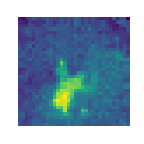
\includegraphics[width=\textwidth]{human.png}
      \caption{Human.}
      \label{fig:first}
  \end{subfigure}
  \begin{subfigure}{0.2\textwidth}
      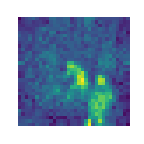
\includegraphics[width=\textwidth]{two-humans.png}
      \caption{Two humans.}
      \label{fig:second}
  \end{subfigure}
  \hfill
  \begin{subfigure}{0.2\textwidth}
      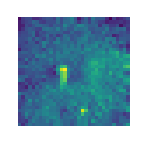
\includegraphics[width=\textwidth]{non-human.png}
      \caption{Non-human heat.}
      \label{fig:second}
  \end{subfigure}
  \begin{subfigure}{0.2\textwidth}
      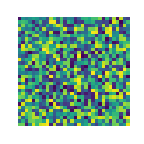
\includegraphics[width=\textwidth]{random.png}
      \caption{Random pixels.}
      \label{fig:third}
  \end{subfigure}
          
  \caption{Different examples of thermal images.}
  \label{fig:sample-frames}
  \end{figure}

\section{Planned methodology}
On an operational level, we apply the \textit{Cross Industry Standard Process for Data Mining} (CRISP-DM) \cite{wirth2000crisp} framework.
This helps us to structure our steps and implies the report structure.
CRISP-DM comprises following steps:
Business understanding, Data understanding, Data preparation, Modeling, Evaluation and Deployment.

\subsection{Data augmentation}
As part of the data preparation step, we augment previously labelled samples.
To enrich the data set, we investigate not only transformation but investigate further methods, as described in \cite{shorten2019survey}.
Ths approach will lead to an increased data set size and may lead to better predictions \cite{perez2017effectiveness}.

\subsection{(State-of-the-Art) ML models}
As first model we evaluate boosted trees (XGBoost) \cite{chen2016xgboost}.
For this approach we construct features as object size, object average temperature, object temperature variation, object movement, etc.

The second model we evaluate is Convolutional Neural Networks (CNN) \cite{lecun1995convolutional}.
The CNN approach shall classify into three categories: (1) No heat-emitting objects, (2) non-human heat-emitting object(s) and (3) human(s).
We might use certain CNN layout, e.g. SqueezeNet \cite{SqueezeNet}.

\subsection{Parameter tuning}
In order to optimize our results we search for promising configuration sets for our models. As discussed during the lecture, a random search approach \cite{bergstra2012random} is state-of-the-art. Previous tuning attempts with Tensorboard were not satisfying. In this project we utilize the Tune framework \cite{liaw2018tune}, which promises advanced parameter optimization opportunities and distributed search possibilities.

% \section{State of the art}
% Read (at least 2) other papers how they have solved similar problem and describe their approach and results. Add citation to other papers.

\bibliographystyle{IEEEtran}
\bibliography{references}

\end{document}
